\documentclass[12pt]{article}
\usepackage{listings}
\usepackage{graphicx}

\begin{titlepage}
    \begin{center}
        \title{ECE 303 Lab Technical Memos}
        \author{Nicholas Sica}
        \date{October 2, 2020}
    \end{center}
\end{titlepage}

\begin{document}
    \maketitle
    \tableofcontents

    \section{Week 1 Lab}
        \subsection{Discussion}
            The point of this lab was to introduce us to the Arduino toolkit and allow anyone who is new to the platform time to adjust and get familiar with the tools presented to them. The lab was straightforward, connect an LED and resistor to a pin on the arduino and writing simplistic code to change the pulse width modulation values. The output is as expected, with the intensity of the light changing based off the number put into the serial monitor, zero being off and 255 being full brightness.
            \begin{figure}[!htb]
                \centering
                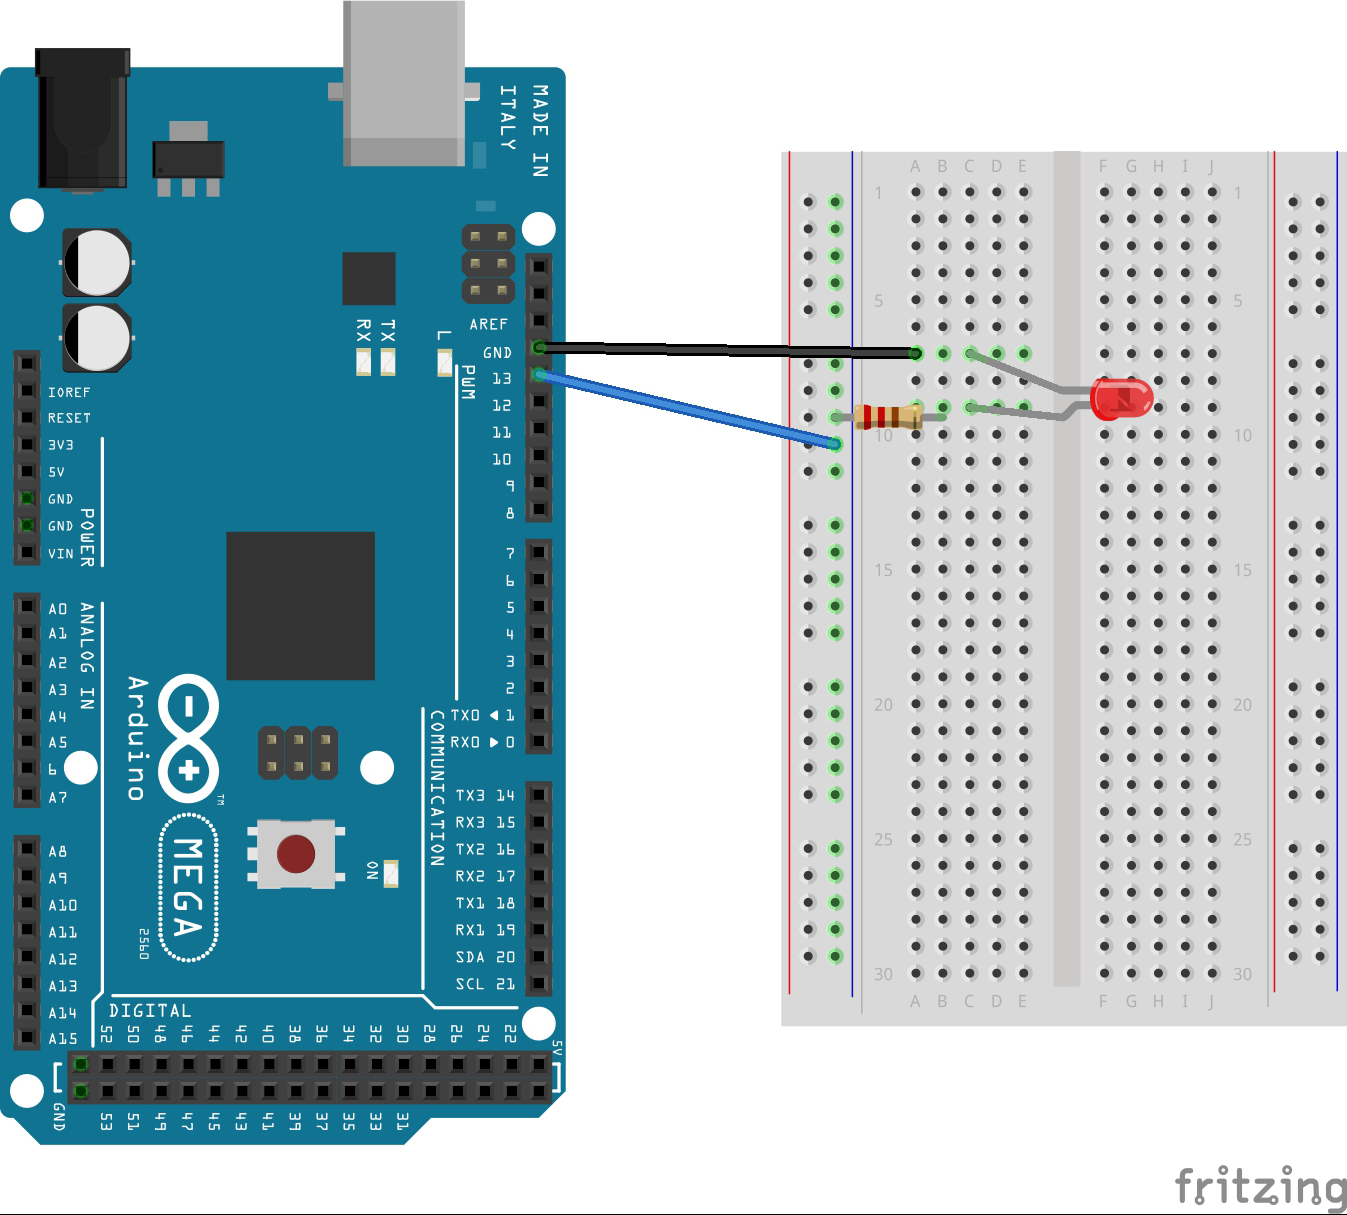
\includegraphics[width=3.0in]{figure_1_1.png}
                \caption{Basic LED Circuit Setup}
                \label{Circuit}
            \end{figure}
        \subsection{Program}
        \lstlisting[language=C++]{../lab_2/src/main.cpp}
\end{document}